\documentclass[tikz,border=4pt]{standalone}
% Estilo común de los diagramas de bloques (se usa con \input en cada standalone)
\usepackage[defaultsans,scale=0.92]{lato}
\usepackage{libertinust1math}
\usepackage{xcolor,amsmath}
\usepackage{tikz}
\usetikzlibrary{positioning,arrows.meta,calc,shapes.geometric}
\usepackage{../../notacion}
\definecolor{ctrlazul}{HTML}{1E5AA8}\definecolor{ctrlnoche}{HTML}{14213D}
\definecolor{ctrlcoral}{HTML}{D1495B}\definecolor{ctrlverde}{HTML}{2A9D8F}
\definecolor{ctrlambar}{HTML}{E09F3E}\definecolor{ctrlgris}{HTML}{5C677D}
\definecolor{ctrlvioleta}{HTML}{6C4AB6}\definecolor{ctrlteal}{HTML}{0F7173}
\tikzset{
  >={Stealth[length=2.4mm]}, every node/.style={font=\small},
  bloque/.style={draw=ctrlnoche,fill=ctrlazul!7,thick,rounded corners=1.5pt,minimum height=9mm,minimum width=13mm,inner sep=4pt},
  suma/.style={draw=ctrlnoche,thick,circle,inner sep=0pt,minimum size=6mm},
  senal/.style={->,thick,draw=ctrlnoche},
  rot/.style={font=\footnotesize,text=ctrlgris},
}

\begin{document}
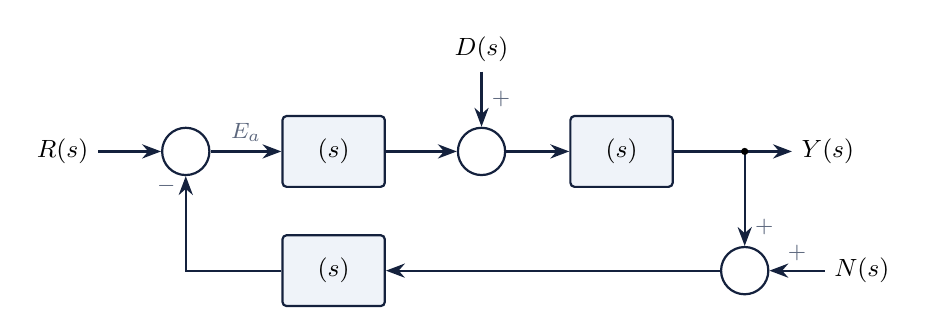
\begin{tikzpicture}
  \node (r) {$R(s)$};
  \node[suma,right=8mm of r] (S) {};
  \node[bloque,right=9mm of S] (C) {$\Gc(s)$};
  \node[suma,right=9mm of C] (S2) {};
  \node[above=7mm of S2] (d) {$D(s)$};
  \node[bloque,right=8mm of S2] (P) {$\Gp(s)$};
  \coordinate[right=9mm of P] (y0);
  \node[right=6mm of y0] (y) {$Y(s)$};
  \node[suma,below=12mm of y0] (S3) {};
  \node[right=7mm of S3] (n) {$N(s)$};
  \node[bloque] (H) at (S3 -| C) {$\Hs(s)$};
  \draw[senal] (r)--(S); \draw[senal] (S)--node[above,rot]{$E_a$}(C); \draw[senal] (C)--(S2);
  \draw[senal] (d)--node[right,rot]{$+$}(S2); \draw[senal] (S2)--(P); \draw[senal] (P)--(y);
  \draw[senal] (y0)--node[right,rot,pos=0.8]{$+$}(S3); \draw[senal] (n)--node[above,rot]{$+$}(S3);
  \draw[senal] (S3)--(H); \draw[senal] (H)-|node[pos=0.95,left,rot]{$-$}(S);
  \fill (y0) circle (1.3pt);
\end{tikzpicture}
\end{document}
